%%
%% Author: jamie
%% 04/10/18
%%

% Document
\chapter{Empirical Studies}\label{ch:empirical}

\section{Overview}\label{sec:empOverview}
In this chapter we will cover a number of experiments that were conducted in order to investigate
the performance of the different algorithms implemented in order to tackle Leduc Hold'em.
We will begin with a simplified version of MCTS for POMDPs and will incrementally add to this
method in order to see how the performance of our agent evolves.
In the table below we have listed the template that we will follow when conduction these experiments.


\addvbuffer[12pt 0pt]{\begin{tabular}[ht]{ | p{2cm} | p{10cm} | }
    \hline
    \textbf{Section} & \textbf{Rationale} \\
    \hline
    Objective & This section will contain an explanation of the purpose of the experiment along with
    how it was carried out \\
    \hline
    Algorithm and Coding & This section will go into the details of the algorithm used to produce results \\
    \hline
    Results & This section will detail the results acquired from the experiments conducted \\
    \hline
    Analysis & In this section we will examine our results and try to provide insight into the
    reasoning behind these results \\
    \hline
\end{tabular}}

\section{Experiment 1 - UCT Versus Random Player}\label{sec:expmeriment1}
The first experiment conducted involved a simplified version of the algorithm outlined in\citep{heinrich2017reinforcement}.
We set an initial goal of using a random player as our benchmark opponent in order to demonstrate how
this algorithm could exploit such a player's strategic inefficiencies.

\subsection{Objective}\label{subsec:objective1}
The goal of this experiment is to implement MCTS for Leduc Hold'em.
The MCTS agent will play against a random player and learn a strategy to exploit this player for
maximal reward.
Although we are interested in the results gained from playing against the random player we treat the
outcome of this experiment as a baseline for our subsequent results.
The reasoning for this is that the difficulty in finding a winning strategy against a random player
is not high.
In fact, at each point in the game that the random player can take an action it is
just as likely to fold it's cards, regardless of their value, as it is to take any other action.
This means that for our agent the intelligent strategy is to merely retain all but the
very worst of its hands.
Thus we can think of the strategy learned by this initial agent as a broad
categorisation between very weak hands and all other hands.
Thus we expect that the exploitability of the resultant agent will be relatively high.
Our agent will not have learned all of the strategic intricacies of the game
and it will not react strategically to the opponent's play.
Rather, it will simply know how to beat a 'dumb' random player.
This will give us a platform to build a more sophisticated agent through different mechanisms such as
self-play in the subsequent experiments.

\subsection{Algorithm and Coding}\label{subsec:algAndCoding1}
As mentioned we will be following Heinrich's implementation.
The pseudocode for this algorithm can be seen in figures 2.4 and 2.5.
This algorithm ticks the box of being applicable to POMDPs like poker.
In our case we are learning values associated with histories of actions and observations that occur in the game.
However it is worth noting that during this first iteration of the algorithm the game tree for only one player had
been implemented and thus did not have to deal with information asymmetry.

\subsection{Results}\label{subsec:results1}
The first metric that was used in order to analyse the results of this experiment is cumulative reward.
This is simply the sum of the output of the reward function over time.
This function directly corresponds to the size of the pot won or lost in the game,
thus the reward can be either positive or negative.
In figure 4.1 we see the reward over time increasing.
In order to obtain these results the algorithm was run for 10,000 iterations and this process was repeated 100 times.
Our cumulative rewards were then averaged at each iteration across these 100 repetitions to give the graph shown.
Figure 4.2 shows the rate of increase of cumulative reward, or the average reward over time.
In the case of figure 4.2 we applied the MCTS algorithm for 500,000 iterations and
repeated this process 20 times, averaging the results.

\begin{figure}[ht]
    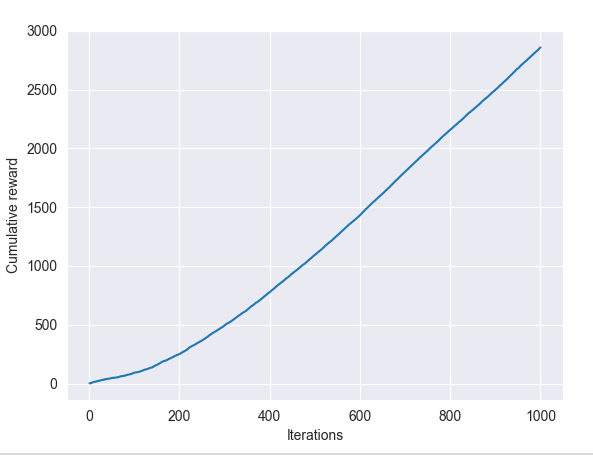
\includegraphics[scale=.8]{images/cumulative_reward_mcts_vs_random.png}
    \caption{MCTS cumulative reward over time vs random player - 10000 Iterations}
\end{figure}

\begin{figure}[ht]
    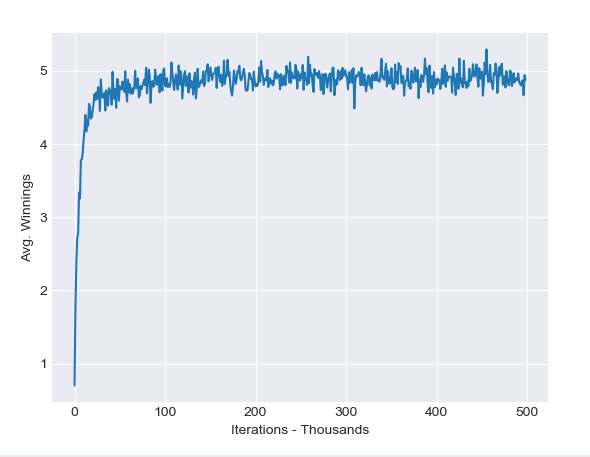
\includegraphics[scale=.7]{images/avg_reward_500000__20_random.png}
    \caption{MCTS slope average reward over time vs random player - 500000 Iterations}
\end{figure}

The second metric used to produce results was exploitability.
This is a measure of the reward that can be gained by playing a best response strategy
against the agent.
In figure 4.3 we see that the exploitability of our agent is quite high throughout, with an
initial dip followed by a divergence towards 4.9.

\begin{figure}[ht]
    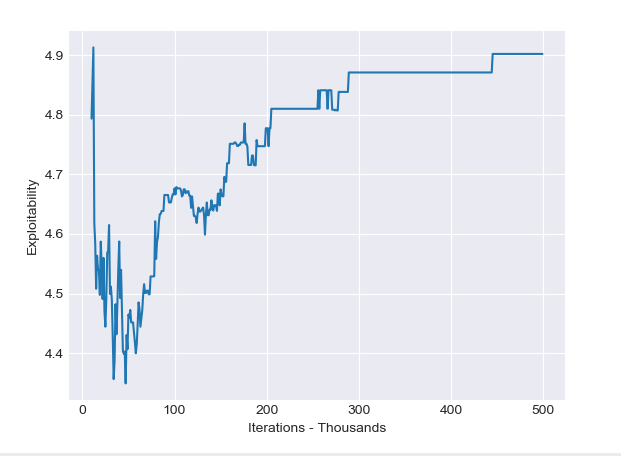
\includegraphics[scale=.7]{images/exploitability_500000_20_random.png}
    \caption{MCTS exploitability over time vs random player - 500000 Iterations}
\end{figure}

\subsection{Analysis}\label{subsec:analysis1}
We will first analyse our results from the cumulative reward metric.
As shown by figure 4.1 we see that initially there is a gradual increase in cumulative reward,
with the slope growing until there is a constant rate of increase.
This demonstrates that during the initial phase of the algorithm we have not yet uncovered
the most beneficial action selection for all states and the exploration phase is still in effect.
However, by visual inspection we can see that over time the rate of increase in cumulative
reward begins to stabilise which indicates that a concrete strategy that can exploit
the random play has been established.
This hypothesis is further supported by figure 4.2 as we see a dramatic upswing
in the rate of increase of cumulative reward followed by a levelling of the graph.

As mentioned the exploitability value throughout this graph is relatively poor with an initial dip followed
by a divergence.
This is most likely explained by the fact that we are not playing against a rational player.
As such our strategy is strong when it comes to maximally exploiting an irrational, random player
but if we then substitute this irrational player for a rational player, the results will not be favourable.

\section{Experiment 2 - UCT Self-Play} \label{sec:experiment2}
In our second experiment the agent was trained against itself.
In other words, two instances of the agent were generated and allowed to develop strategies
through self-play.

\subsection{Objective}\label{subsec:objective2}
The objective of this experiment was to implement Heinrich's extensive form MCTS using UCB action
selection (ie extensive form UCT).
Here a significant improvement in the exploitability of the agent was expected.
This was due to the fact that the opposing agent is rational, in that it learns
through experience.


\subsection{Algorithm and Coding}\label{subsec:algAndCoding2}
\subsection{Results}\label{subsec:results2}
In the case of self-play both agents develop intelligent strategies.
This means that we do not see any significant trends in cumulative reward or average reward over time
due to the fact that neither player has an advantage.
As such these metrics were disregarded and exploitability became the sole metric.
Once again we applied the algorithm for 500,000 iterations, repeating this process 10 times
and averaging the results.

In figure 4.4 it can be seen that there is a notable improvement in exploitability, with lows of 3.5 initially
but over time the values begin to diverge once again back towards 4.6.

\begin{figure}[ht]
    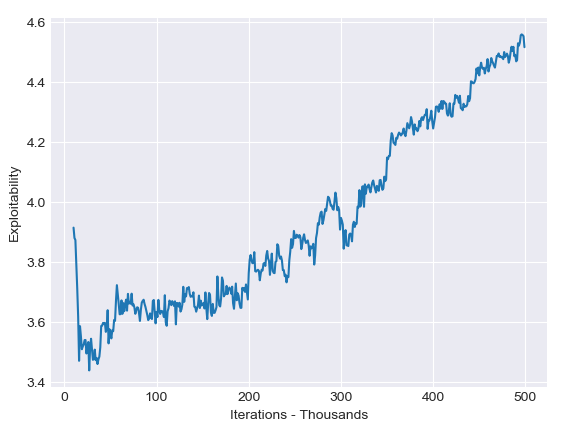
\includegraphics[scale=.7]{images/exploitability_self-play_deterministic_500000.png}
    \caption{MCTS exploitability over time vs random player - 500000 Iterations}
\end{figure}

\subsection{Analysis}\label{subsec:analysis2}
The results gleaned from this experiment were unexpected to a degree.
Heinrich had shown exploitability reaching lows of .8 and diverging to 1.5 in a similar experiment.
Although a similar trend was shown here our exploitability values were significantly higher.
This could potentially be explained by differences in the algorithm used to calculate exploitability
or the implementation of UCT itself.

On further inspection of the search trees generated, along with the best response tree (see chapter 3)
there appeared to be an over-fitting to the opponents strategy over time.
Notably, both instances of the agent were playing more conservatively than expected.
This meant that the best-response player could regularly force our agent to fold in
situations where folding against a less conservative player would be illogical.
In order to conceptualize this phenomenon the following example is given.
Let's say player one is very conservative and they decide to only raise in the second round of the game when they
have a pair of aces.
This means that over time player two will only receive highly negative rewards for the states in
which player one has raised in the second round.
In fact, in this case it is more beneficial for player two to simply fold if player one raises in
the second round of the game.
When a new player is introduced to the system however, they can take advantage of this
behavior by simply raising more frequently in the second round of the game.
This type of strategic feedback loop is characteristic of deterministic strategies due to the
fact that breaking such a loop becomes less and less likely the closer we get to purely greedy action selection.


\section{Experiment 3 - Smooth UCT}\label{sec:experiment3}

\subsection{Objective}\label{subsec:objective3}
\subsection{Algorithm and Coding}\label{subsec:algAndCoding3}
\subsection{Results}\label{subsec:results3}
\subsection{Analysis}\label{subsec:analysis3}

